\documentclass[text01.tex]{subfiles}
\begin{document}
%
% section 1.3
%
\section{ラズベリーパイになれよう（2）}

%
% subsection 1.3.1
%
\subsection{写真をさつえいしよう}

%
% subsubsection 1
%
\subsubsection{ウェブカメラで写真をさつえいしよう}
\hrule\vspace*{5mm}

ウェブカメラを使用して\ruby{画像}{がぞう}をさつえいします。
まずは、ラズベリーパイにウェブカメラを\ruby{接続}{せつぞく}しましょう。
マウスと同じように、ウェブカメラのUSBたんしをラズベリーパイのUSBたんしに差し\ruby{込}{こ}みます。
%
\begin{figure}[htbp]
  \centering
  % 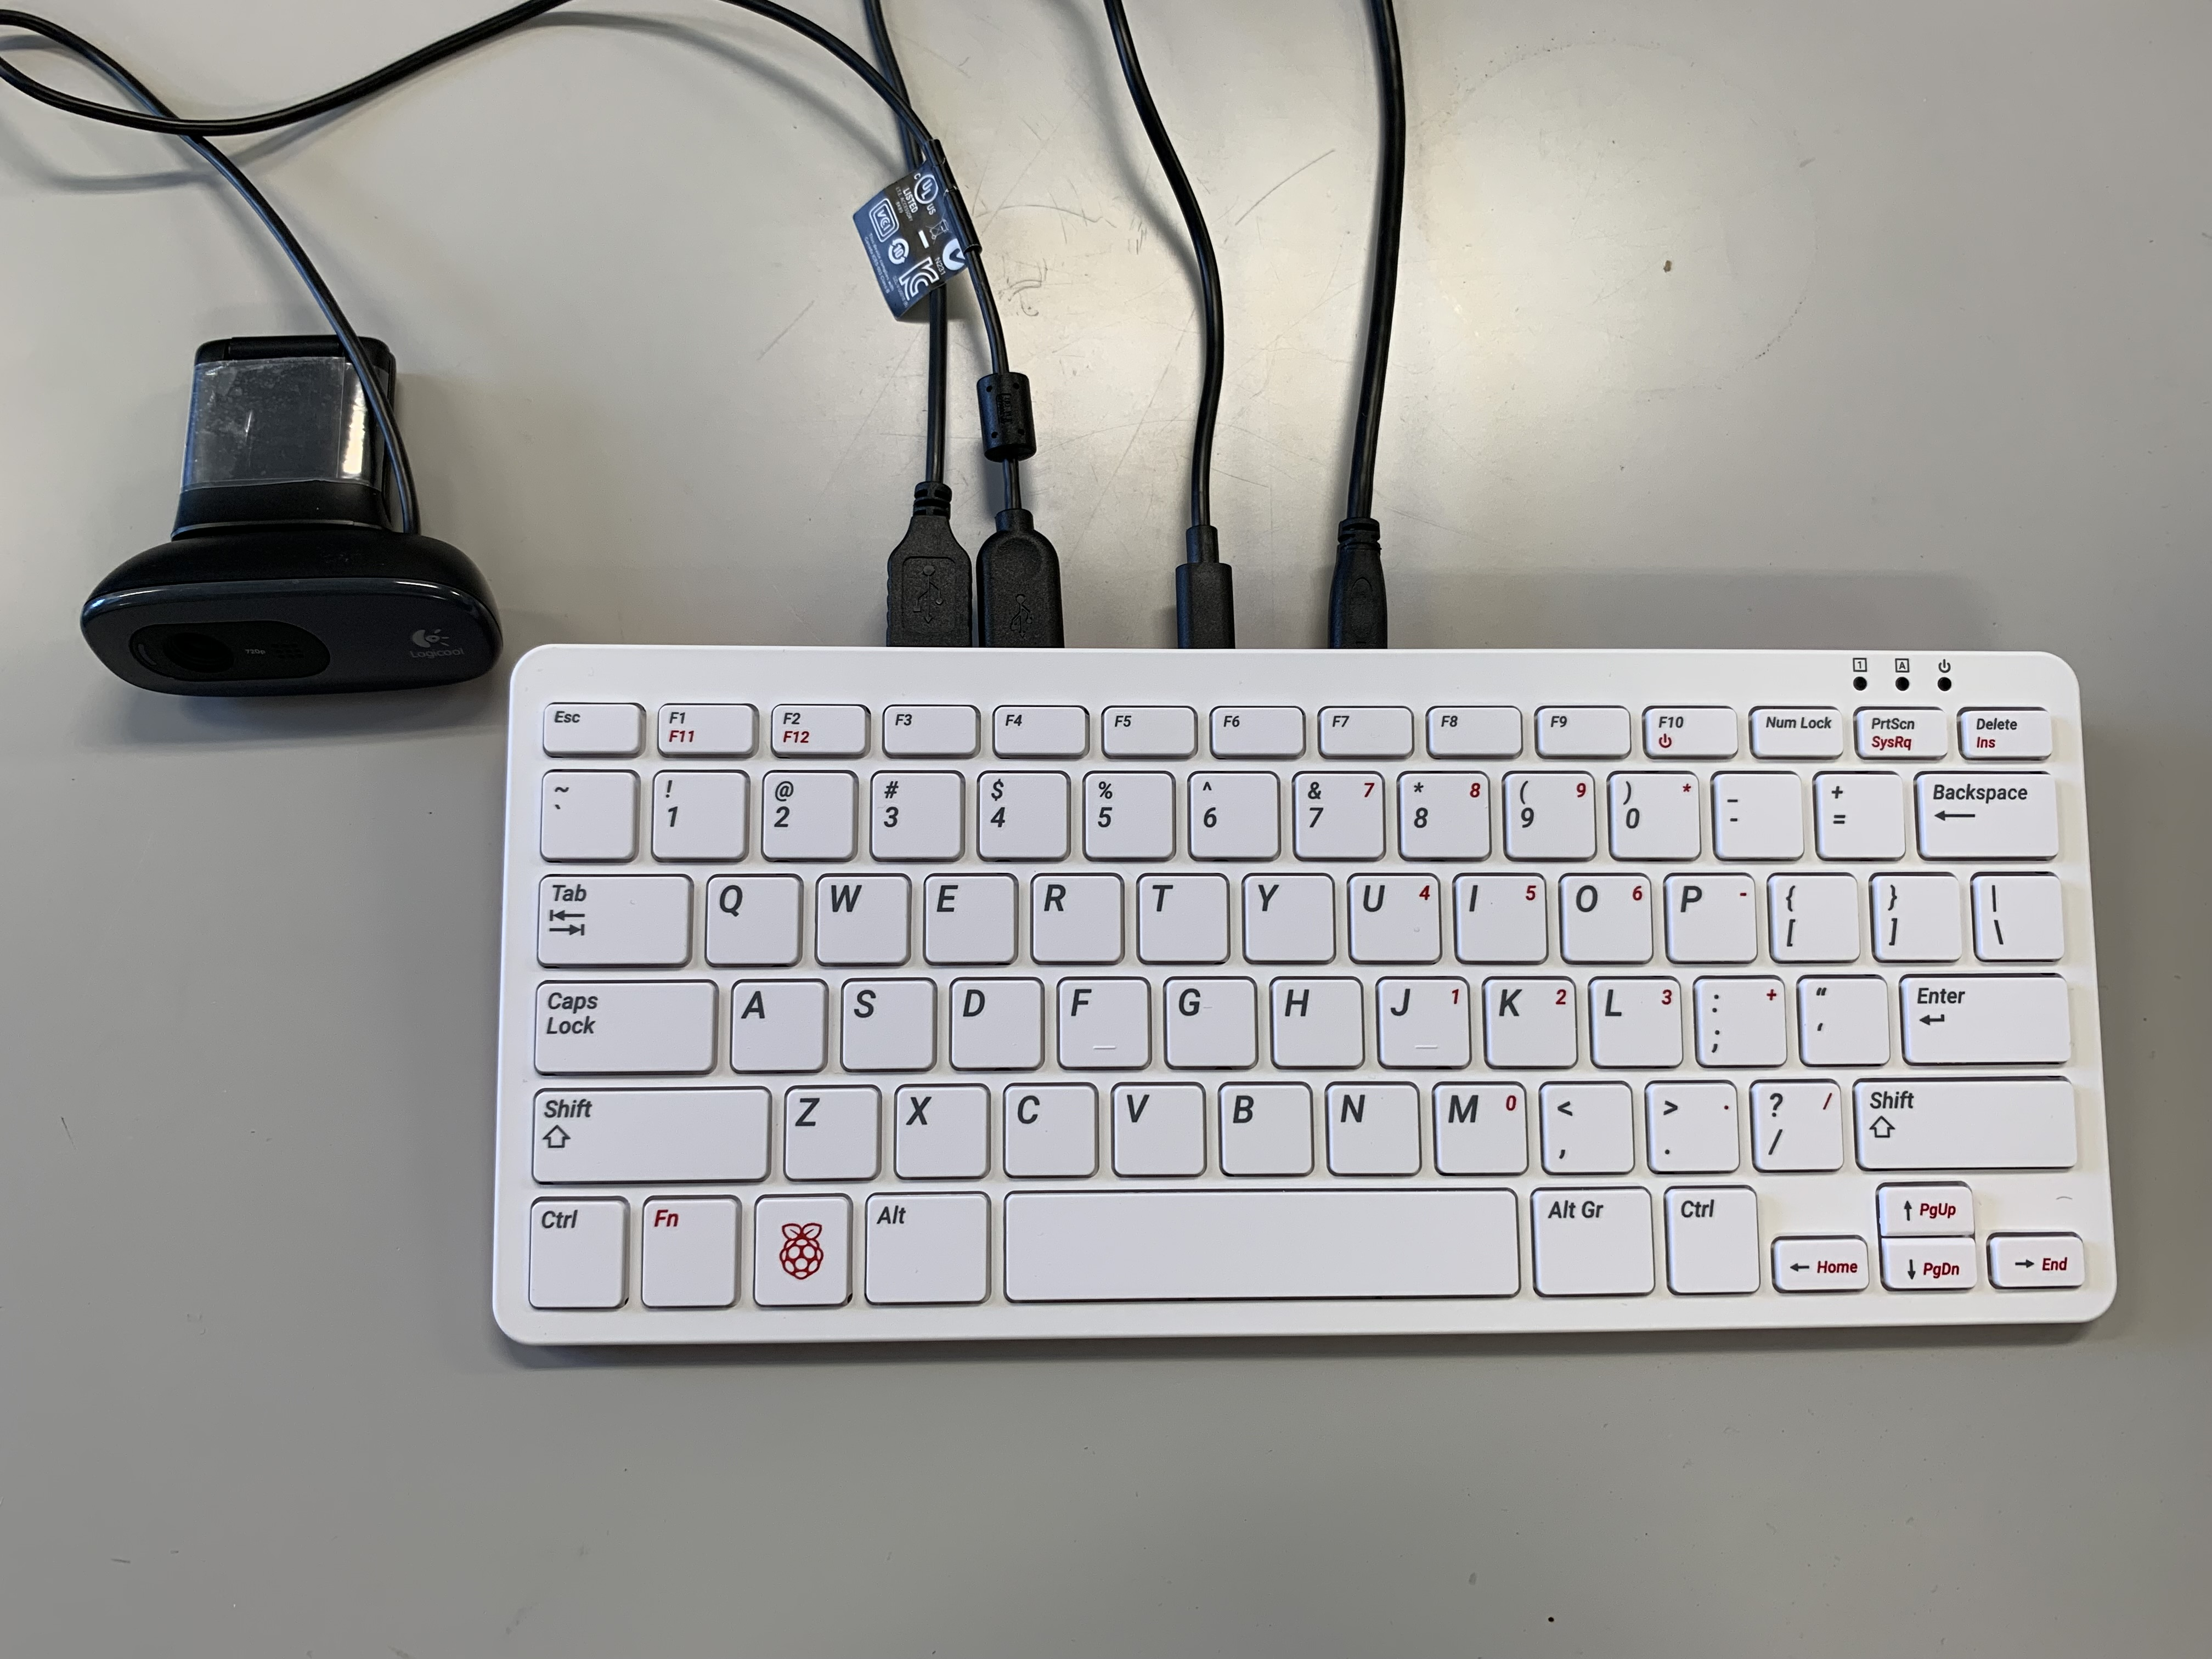
\includegraphics[keepaspectratio, height=30mm]{../../asset/image/textbook-img112-2023.jpg}
  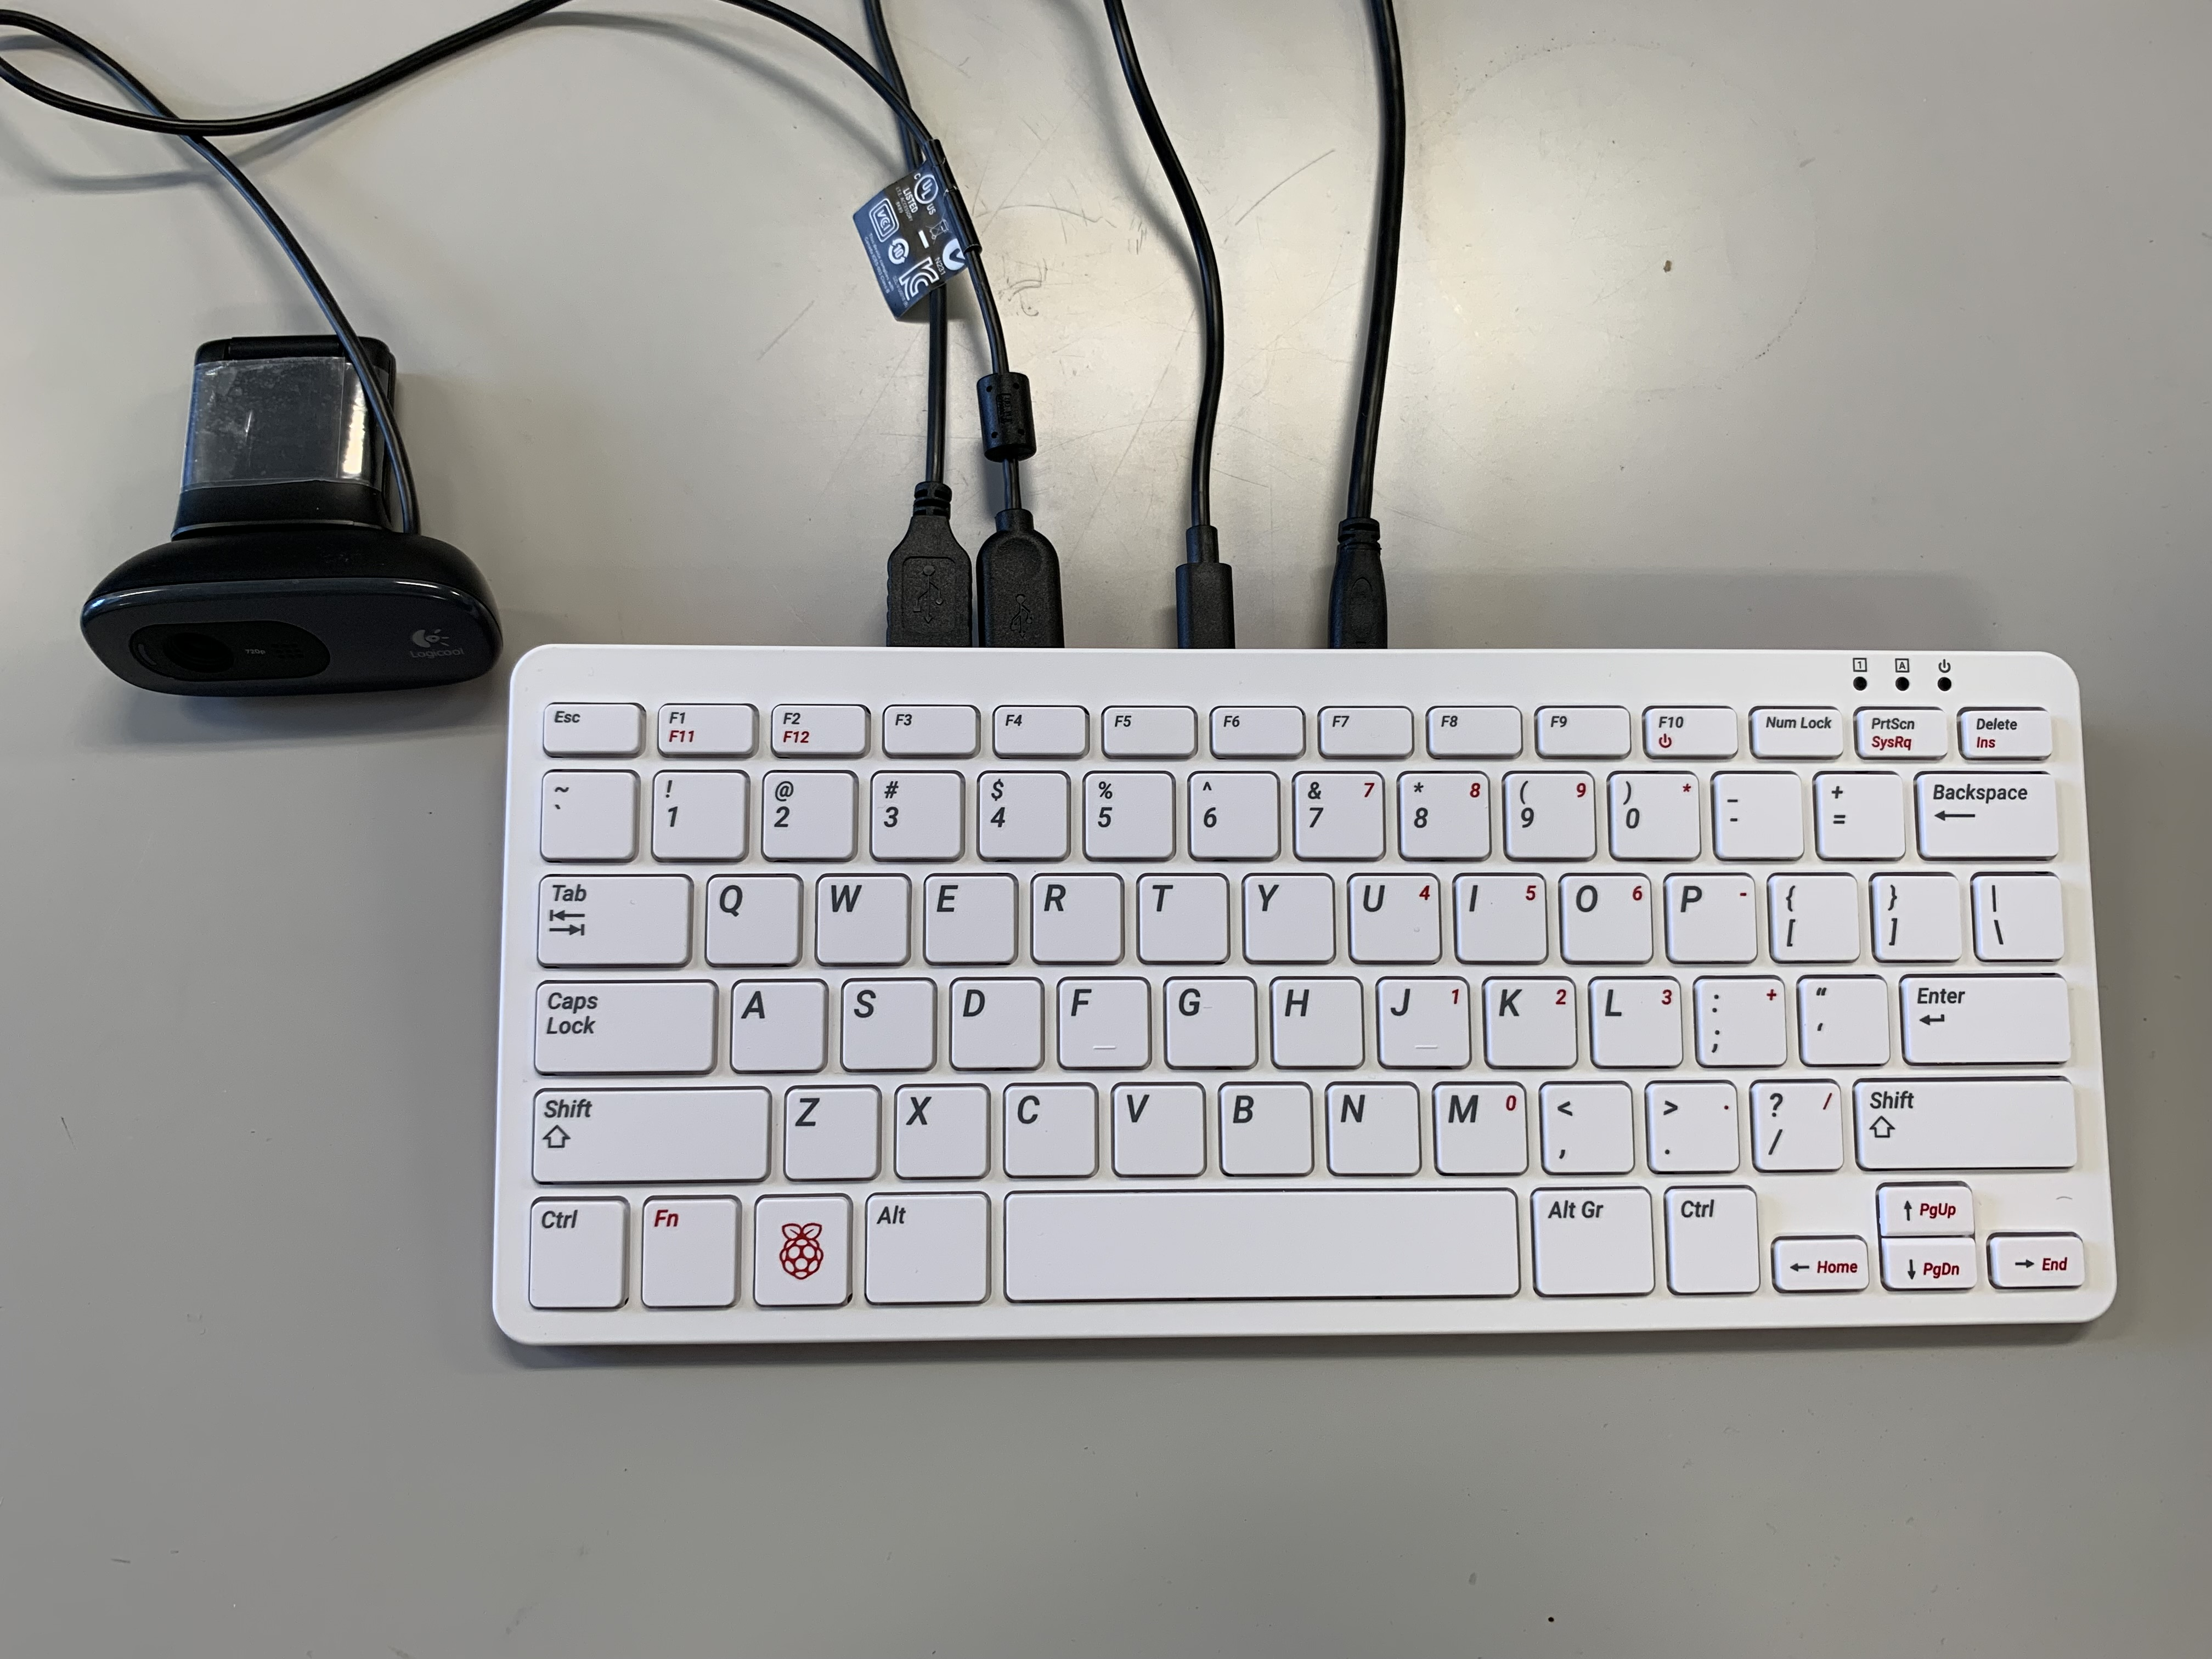
\includegraphics[keepaspectratio, width=0.5\linewidth]{../../asset/image/textbook-img112-2023.jpg}
  \caption{Webカメラの\ruby{接続}{せつぞく}}
  \label{fig:1.3.1}
\end{figure}

ウェブカメラを\ruby{接続}{せつぞく}したら、ラズベリーパイからウェブカメラの\ruby{画像}{がぞう}を取得してみましょう。
左上のラズベリーのアイコンをクリックします。
そこから、サウンドとメディアを\ruby{選択}{せんたく}して、VLCメディアプレイヤーをクリックします。
%
\begin{figure}[htbp]
  \centering
  % 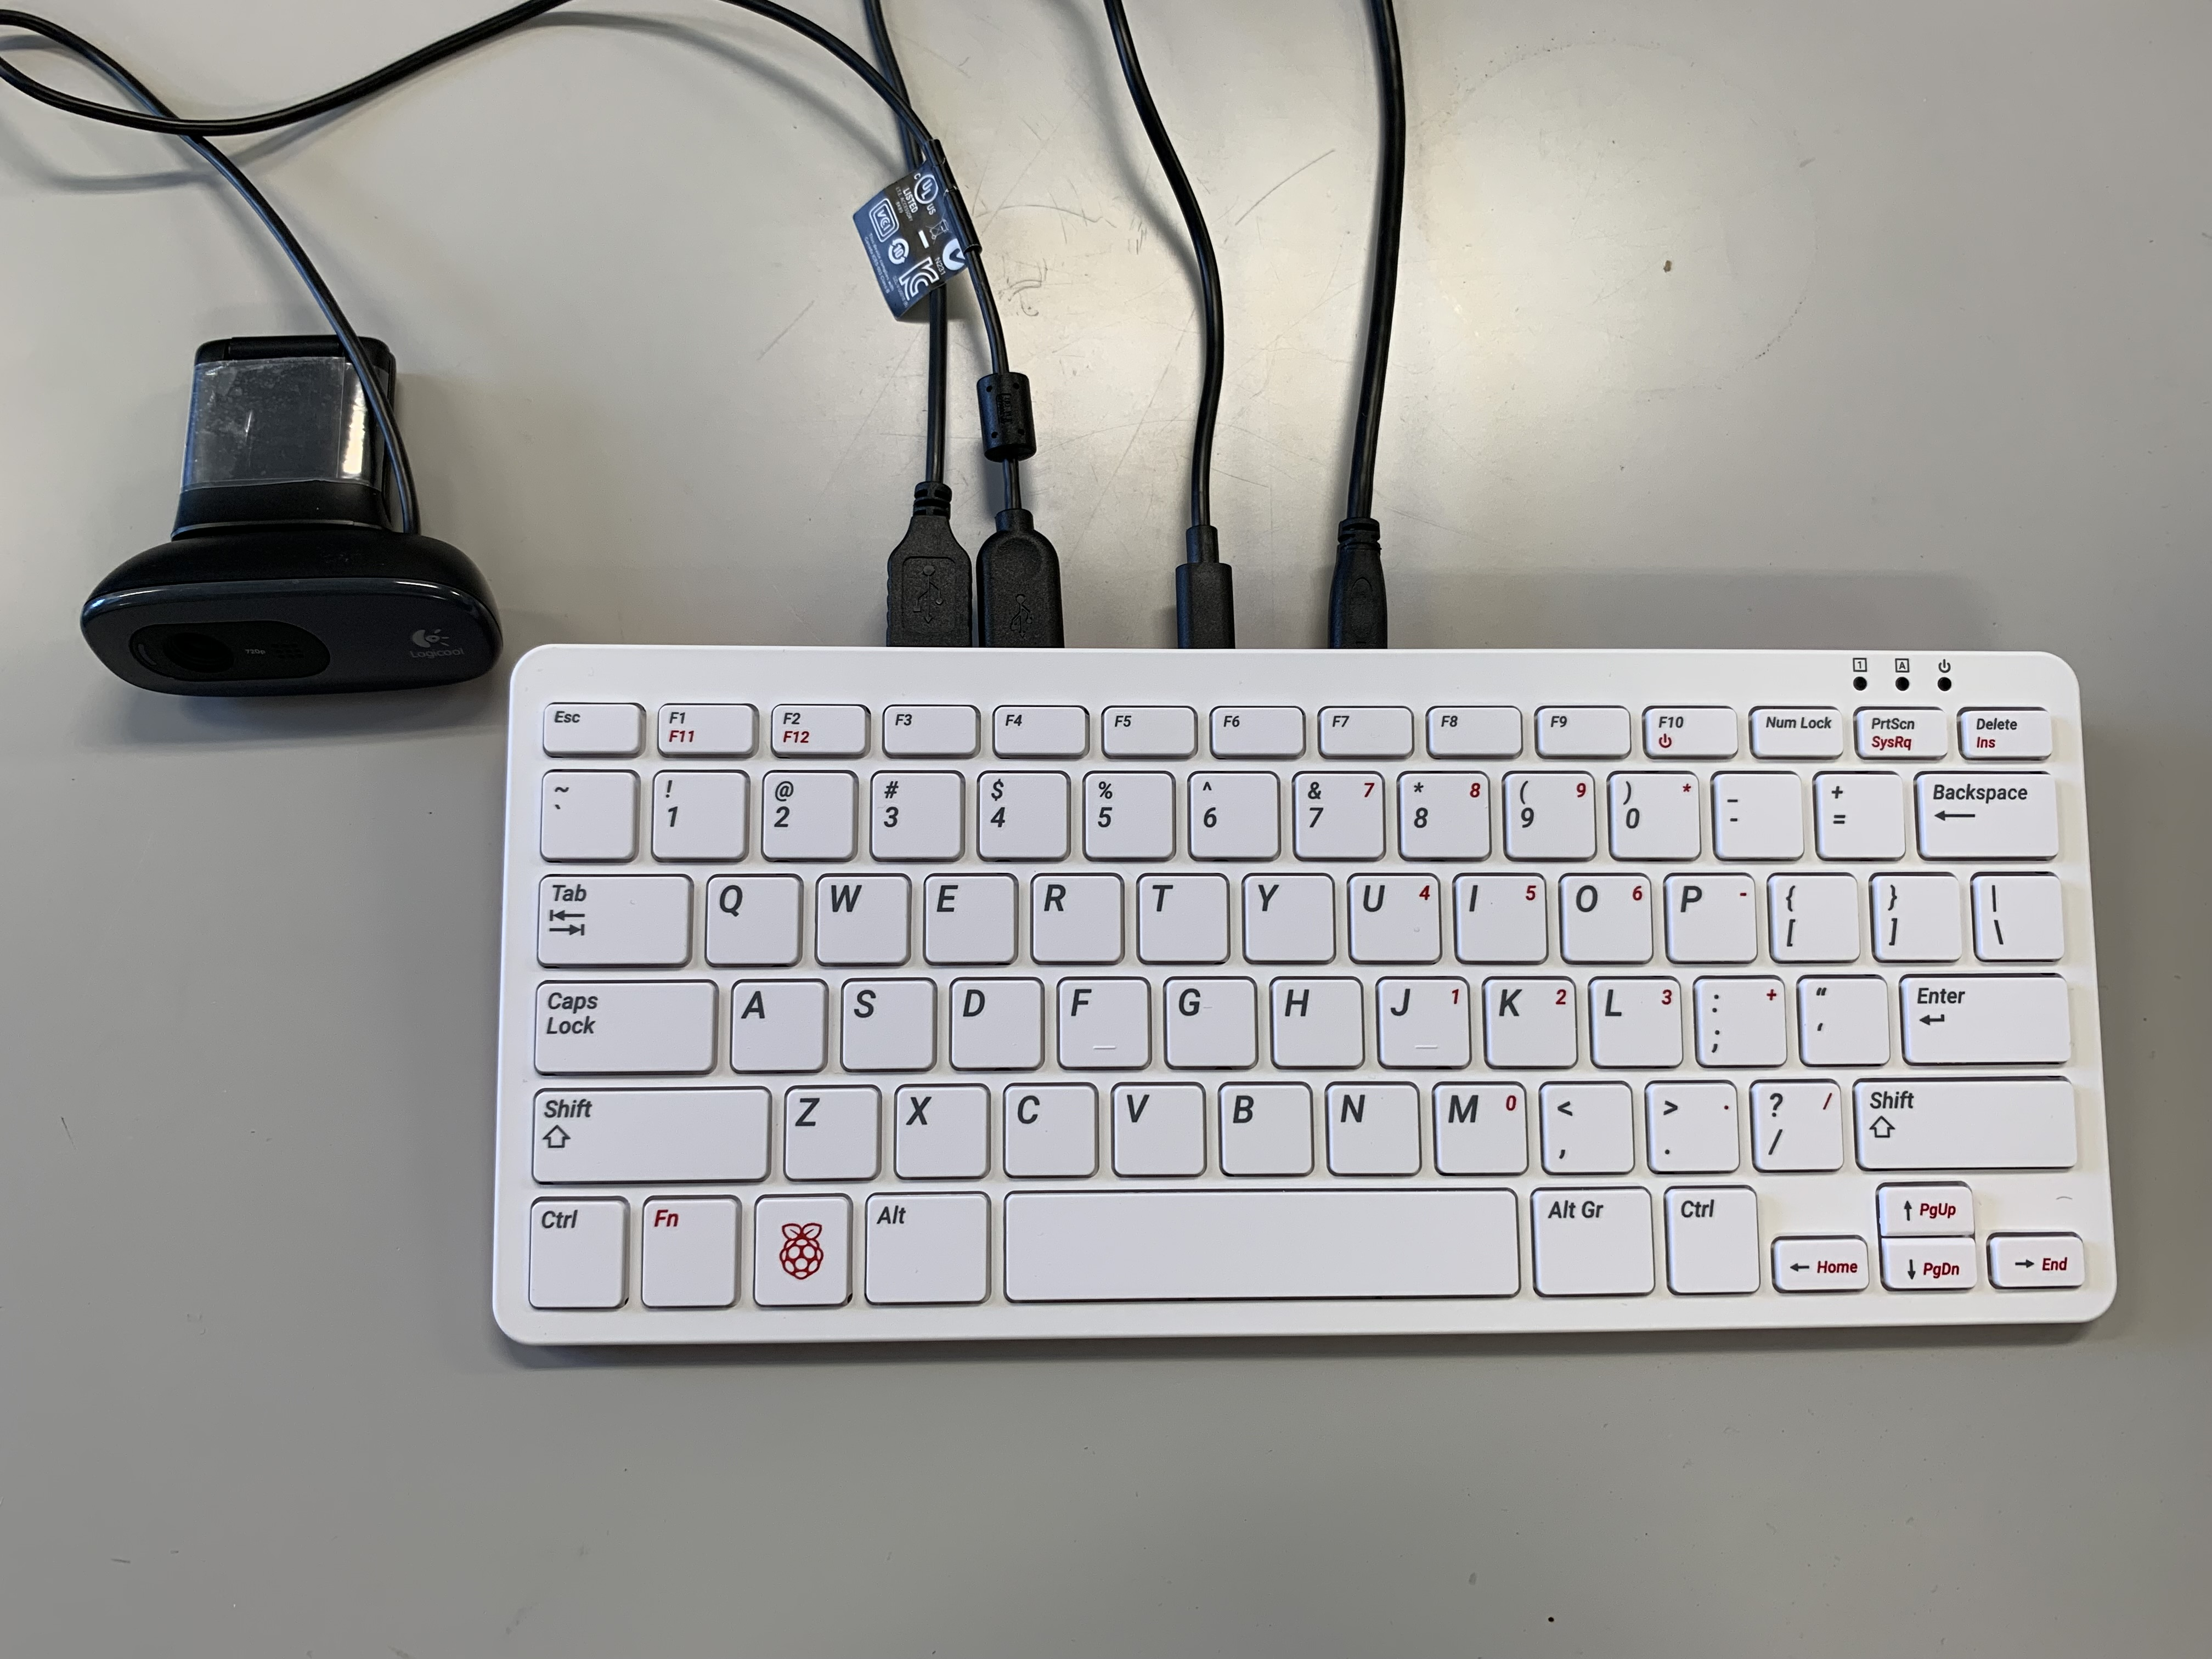
\includegraphics[keepaspectratio, height=30mm]{../../asset/image/textbook-img112-2023.jpg}
  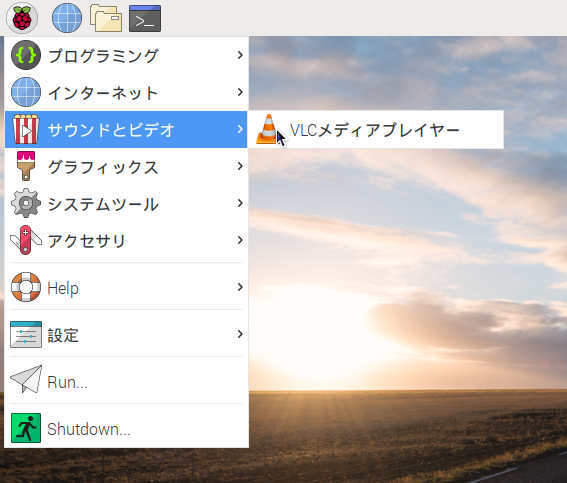
\includegraphics[keepaspectratio, width=0.5\linewidth]{../../asset/image/textbook-img113.png}
  \caption{VLCの起動}
  \label{fig:1.3.2}
\end{figure}
\clearpage

\noindent%
次の図のように、VLCメディアプレーヤーが起動します。
%
\begin{figure}[htbp]
  \centering
  % 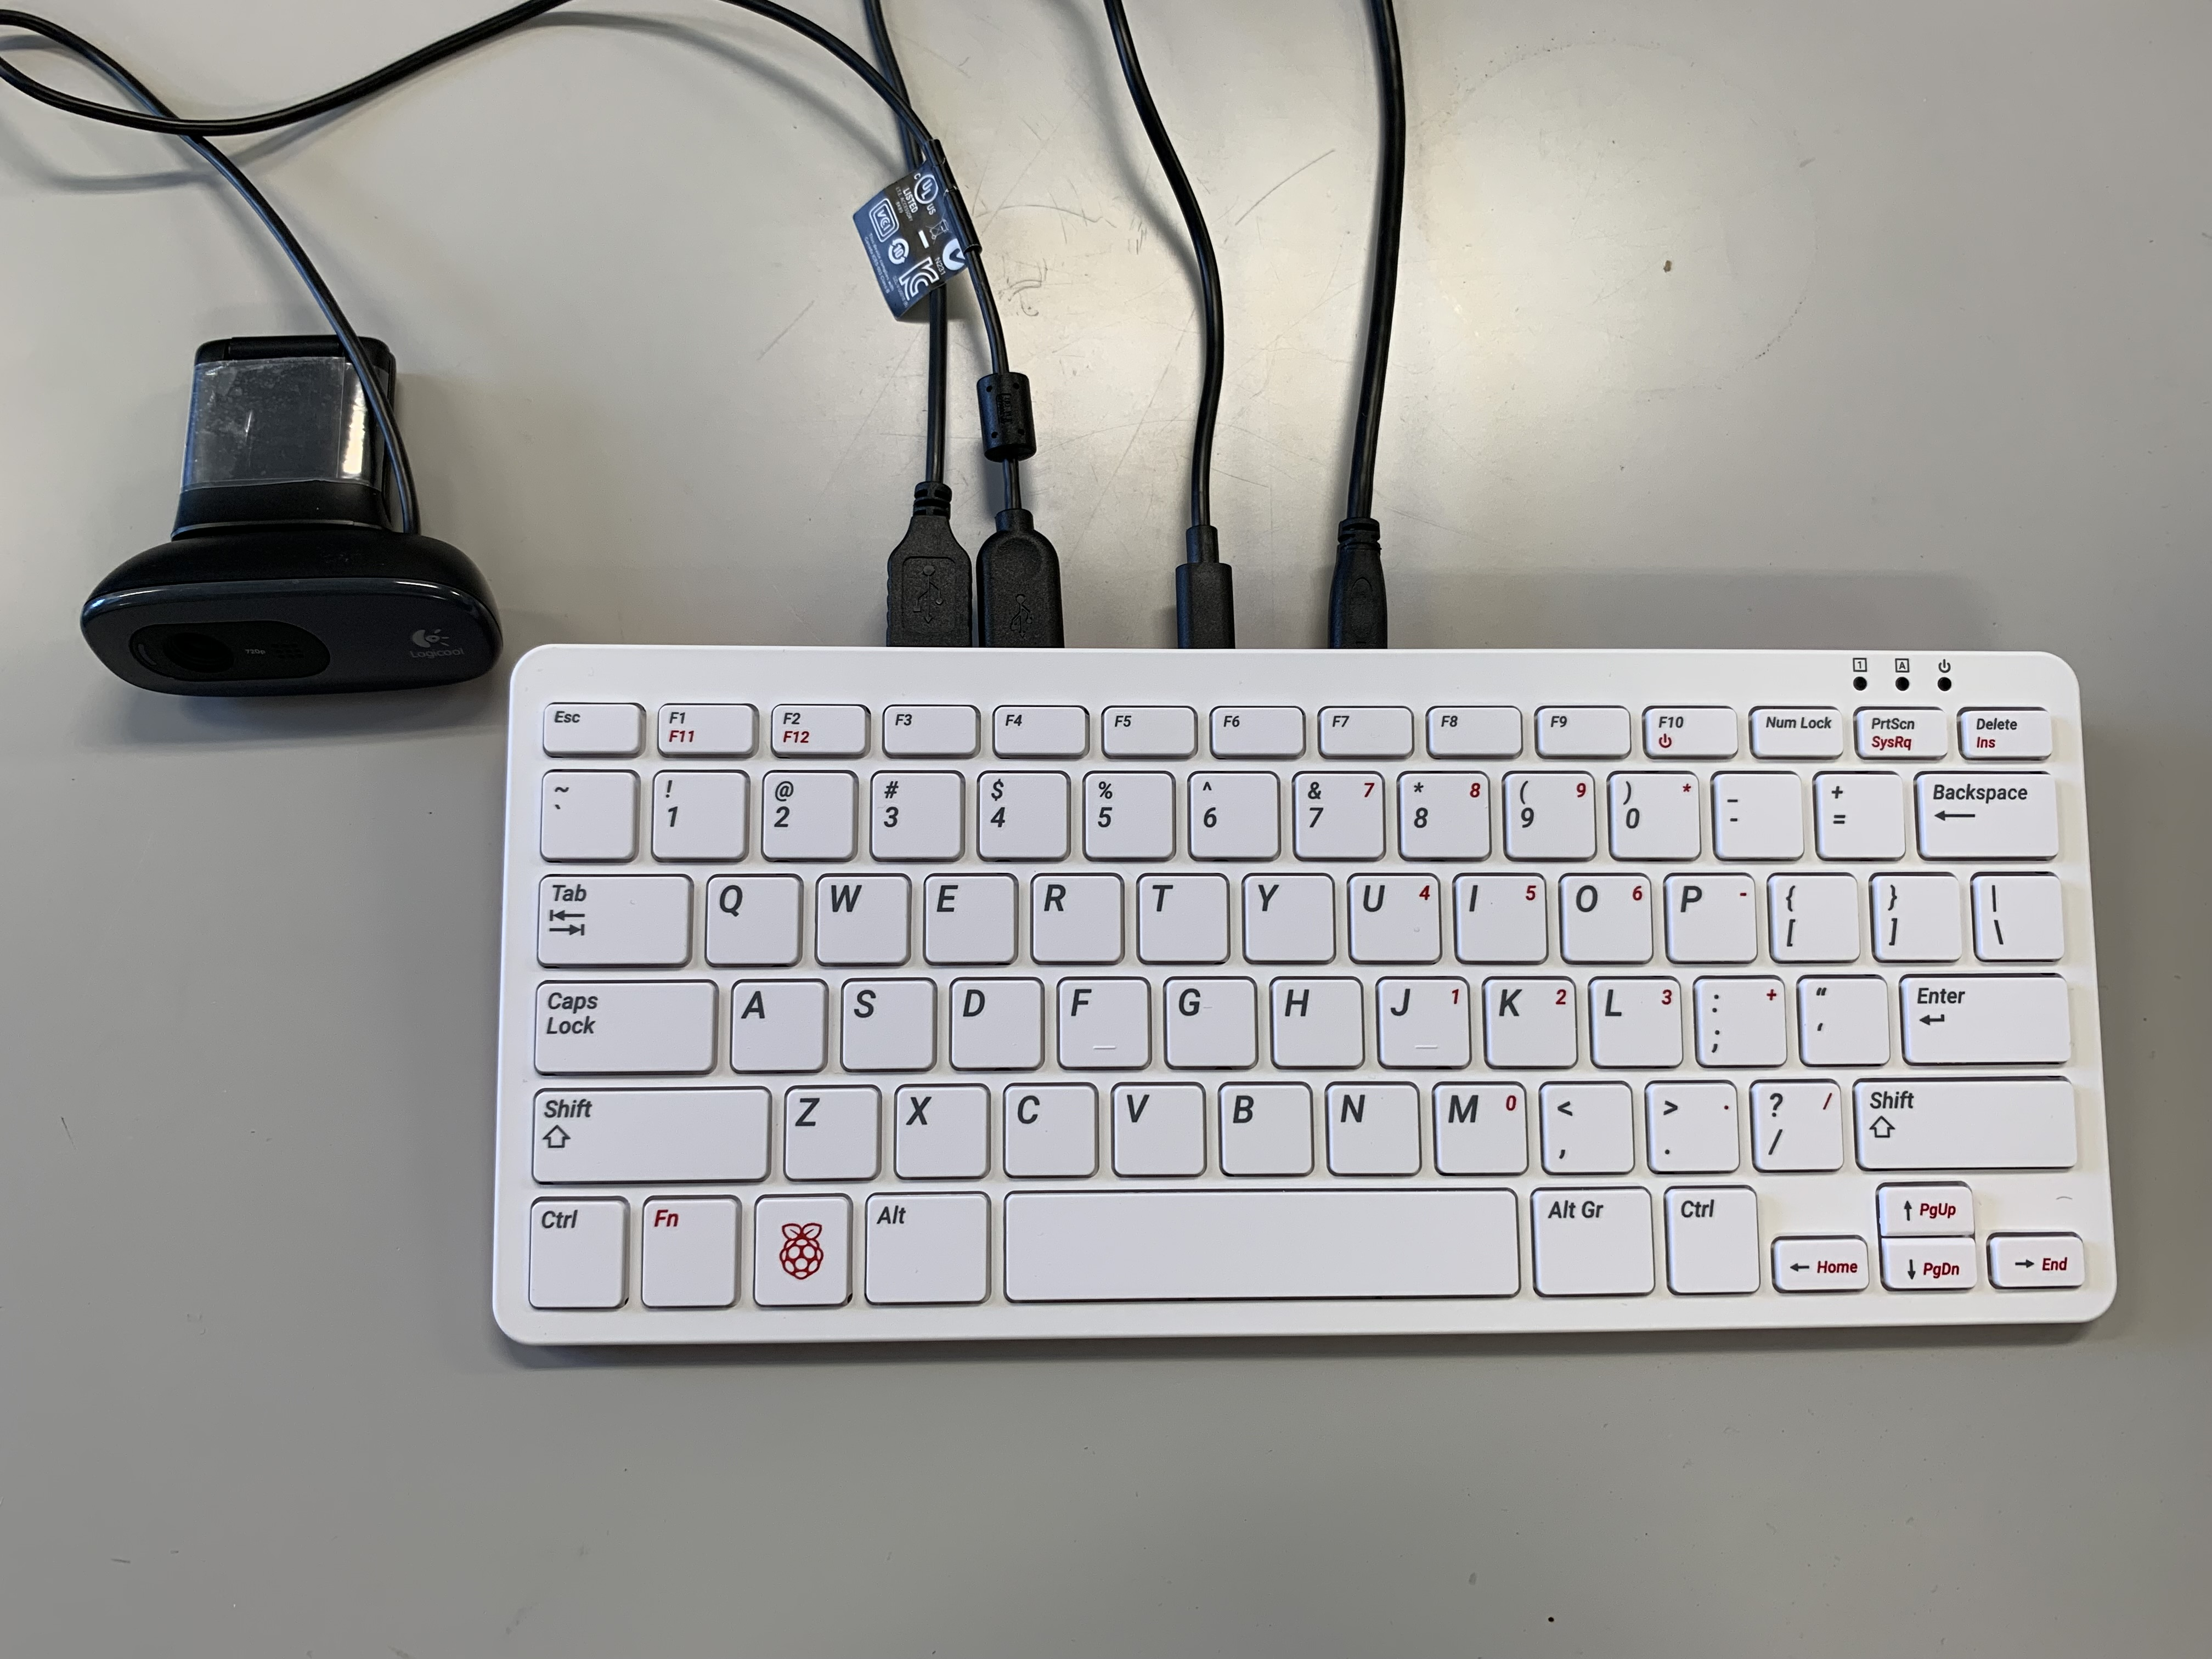
\includegraphics[keepaspectratio, height=30mm]{../../asset/image/textbook-img112-2023.jpg}
  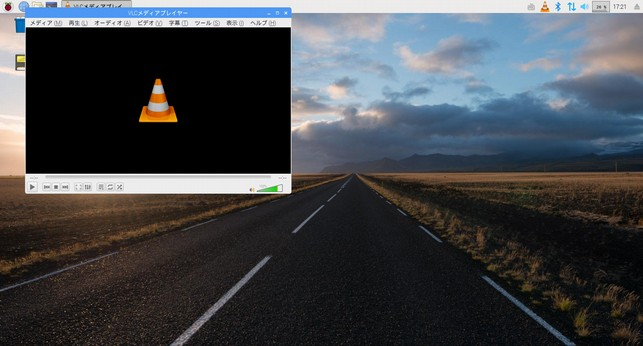
\includegraphics[keepaspectratio, width=0.5\linewidth]{../../asset/image/textbook-img114.jpg}
  \caption{VLC}
  \label{fig:1.3.3}
\end{figure}

次に、Webカメラの映像を、VLCメディアプレイヤーに表示させます。
VLCメディアプレイヤーの「メディア」メニューから、「キャプチャーデバイスを開く」をクリックします。
%
\begin{figure}[htbp]
  \centering
  % 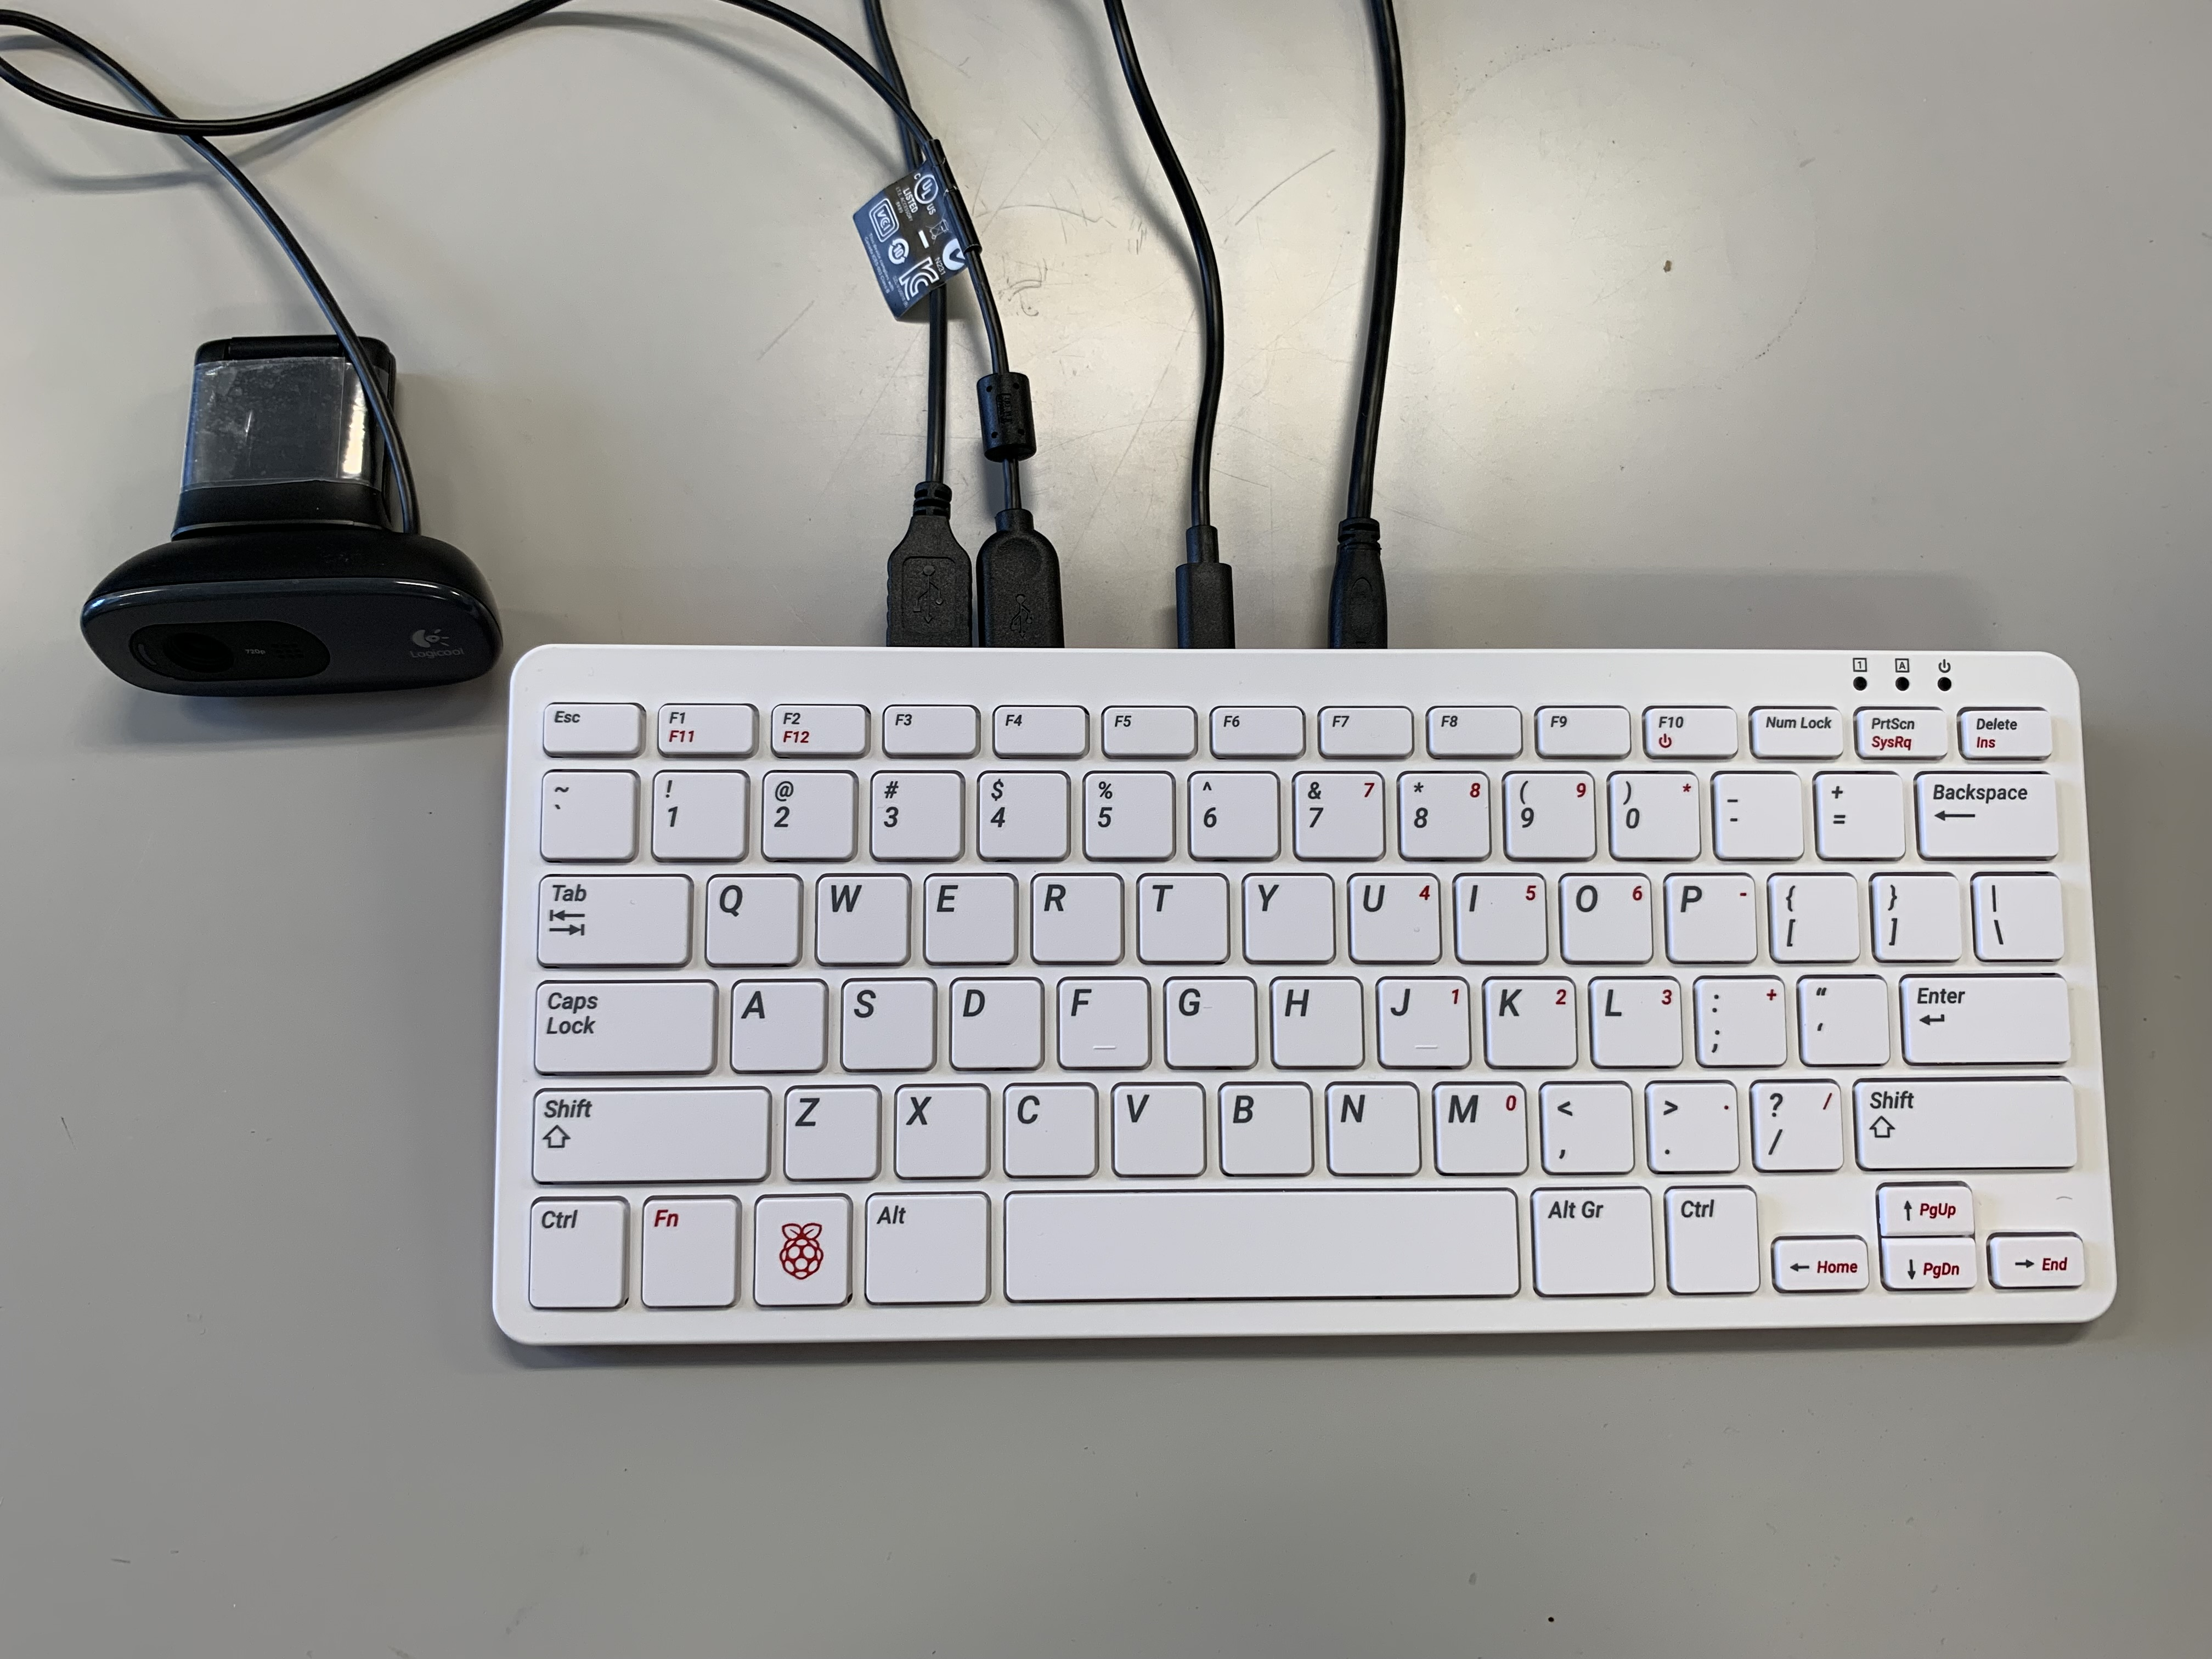
\includegraphics[keepaspectratio, height=30mm]{../../asset/image/textbook-img112-2023.jpg}
  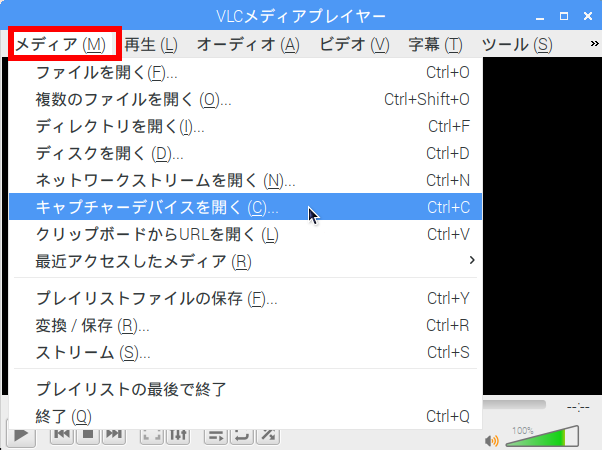
\includegraphics[keepaspectratio, width=0.5\linewidth]{../../asset/image/textbook-img116.png}
  \caption{キャプチャデバイスを開く}
  \label{fig:1.3.4}
\end{figure}

「メディアを開く」ウィンドウの赤線で囲われている「キャプチャーモード」を
「Video camera」にして、青線で囲われている「\ruby{再生}{さいせい}」ボタンをクリックします。
%
\begin{figure}[htbp]
  \centering
  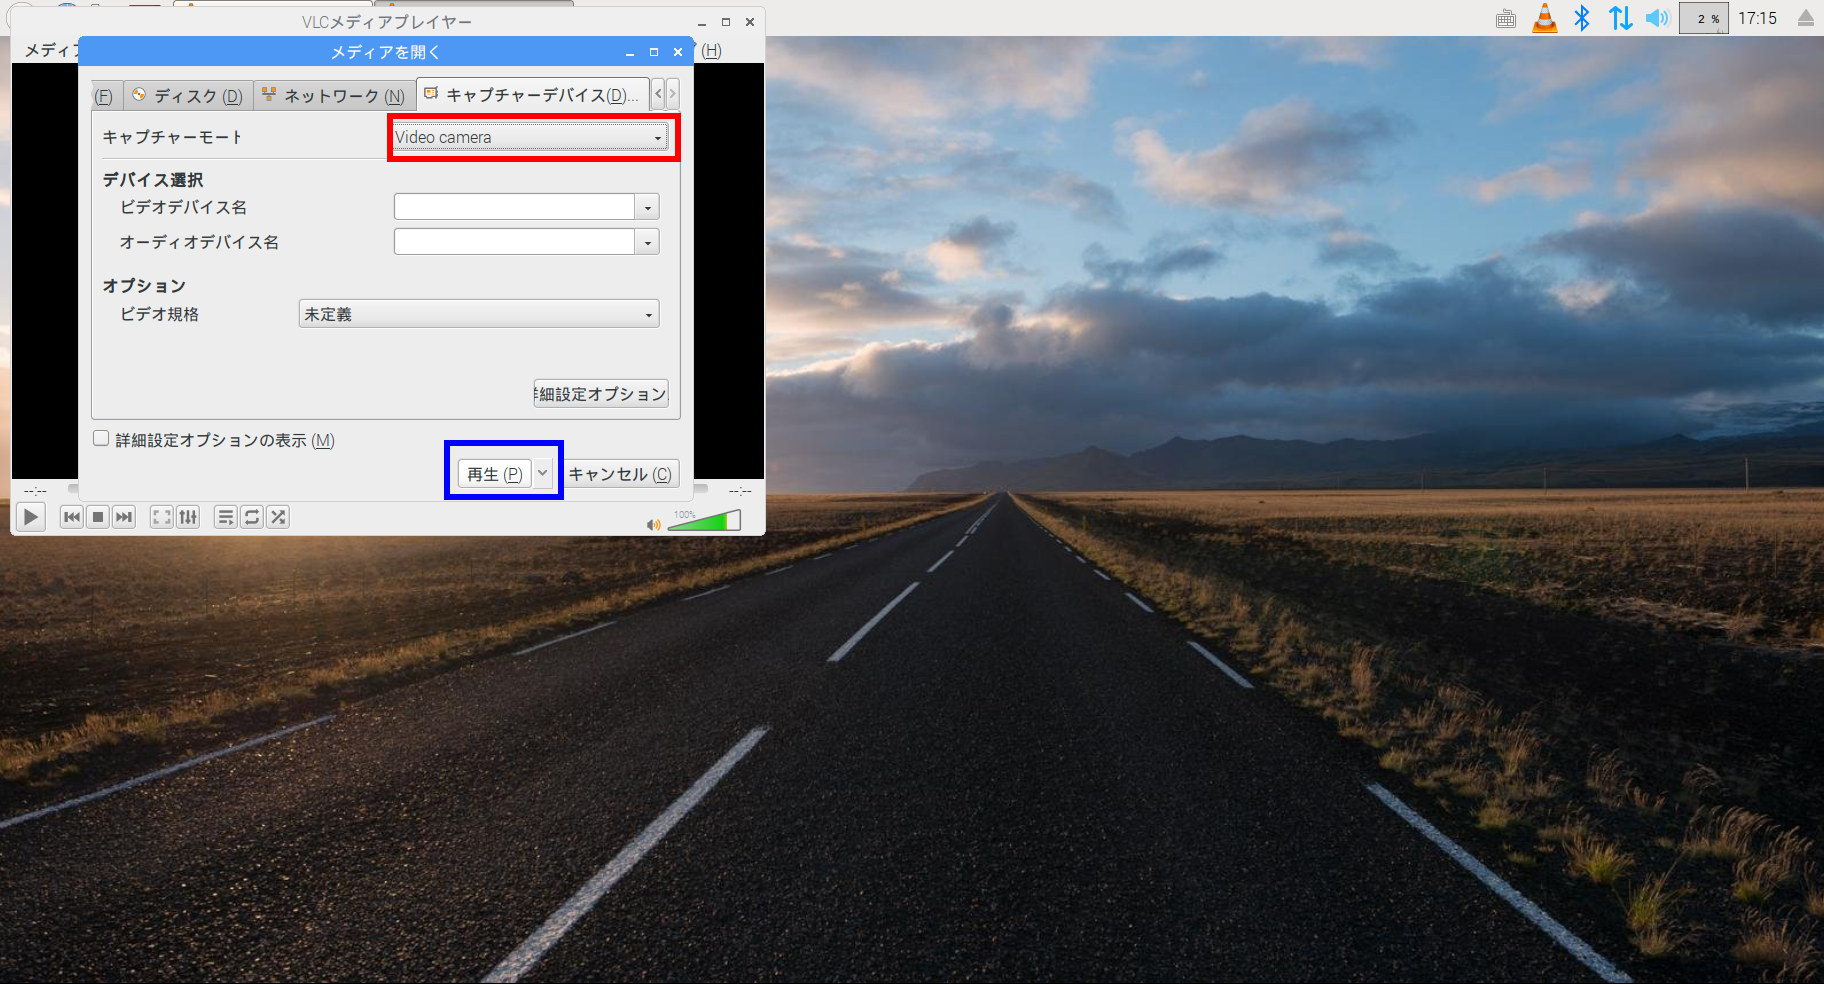
\includegraphics[keepaspectratio, width=0.5\linewidth]{../../asset/image/textbook-img117.png}
  \caption{Webカメラの選択}
  \label{fig:1.3.5}
\end{figure}

\noindent%
しばらくすると、Webカメラからの映像が画面に表示されます。
\clearpage

次に、カメラでさつえいしてみましょう。
「ビデオ」メニューから、「スナップショットを撮る」をクリックします。
%
\begin{figure}[htbp]
  \centering
  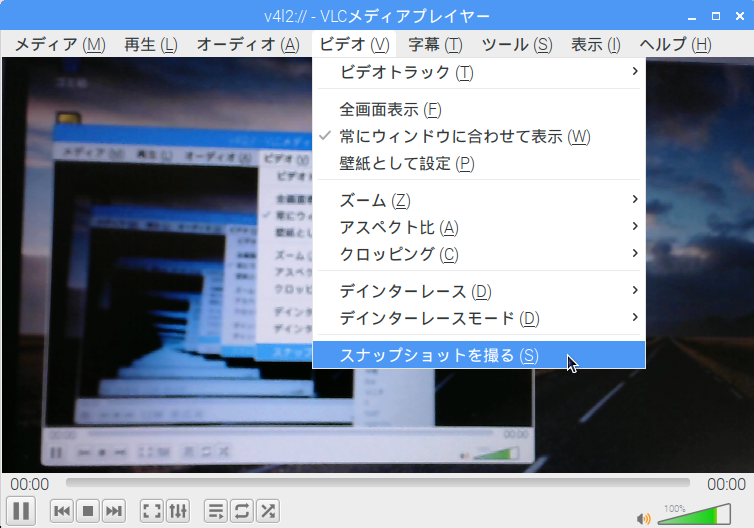
\includegraphics[keepaspectratio, width=0.5\linewidth]{../../asset/image/textbook-img118.png}
  \caption{スナップショット}
  \label{fig:1.3.6}
\end{figure}

\noindent%
下の図のように、保存場所が画面上部に表示されます。
スナップショット画像は、その場所に自動的に保存されます。
%
\begin{figure}[htbp]
  \centering
  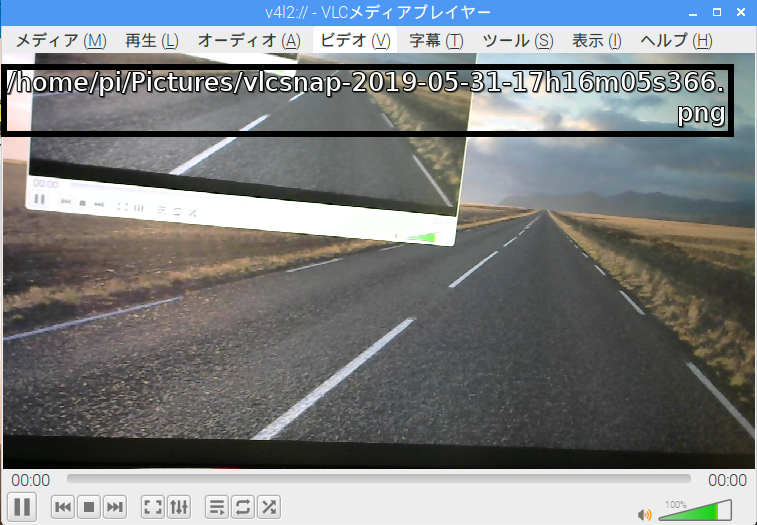
\includegraphics[keepaspectratio, width=0.5\linewidth]{../../asset/image/textbook-img120.png}
  \caption{スナップショット画像の保存}
  \label{fig:1.3.7}
\end{figure}

\noindent%
通常は、Picturesフォルダの下に保存されますので、確認してみましょう。
\bigskip

\begin{tcolorbox}[title=\useOmetoi,breakable]
  \begin{enumerate}
    \addex{同じグループのお友達やティーチングアシスタントの先生のスナップショットを撮ってみましょう。}
  \end{enumerate}
\end{tcolorbox}
\clearpage

%
% subsubsection 1
%
\subsubsection{\ruby{画像}{がぞう}に絵をかこう}
\hrule\vspace*{5mm}

ここでは、\ruby{画像}{がぞう}を\ruby{編集}{へんしゅう}できるアプリケーション「GIMP」を使って、
色付きの筆で自分の顔写真に絵をかきましょう。
GIMPで\ruby{画像}{がぞう}を開いて、色を\ruby{選択}{せんたく}して、筆を選んでから、絵をかいていきます。
\vspace{0.3cm}

{\bf 手順}
\vspace{0.3cm}

  \begin{minipage}{0.4\textwidth}
    \centering
    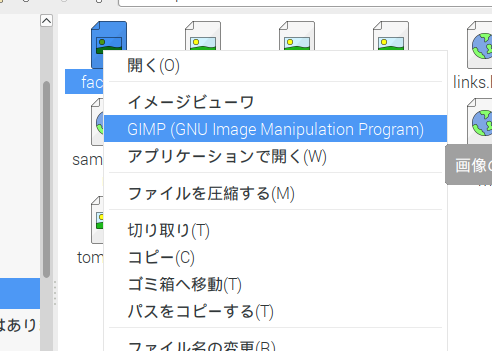
\includegraphics[width=\linewidth]{../../asset/image/textbook-img124.png}\\
    \flushleft
    \textcircled{\scriptsize{1}} %
    \ruby{編集}{へんしゅう}したい\ruby{画像}{がぞう}ファイルを右クリックして、【次で開く】→【GIMP】をクリック
  \end{minipage}
  \hspace{2cm}
  \begin{minipage}{0.4\textwidth}
    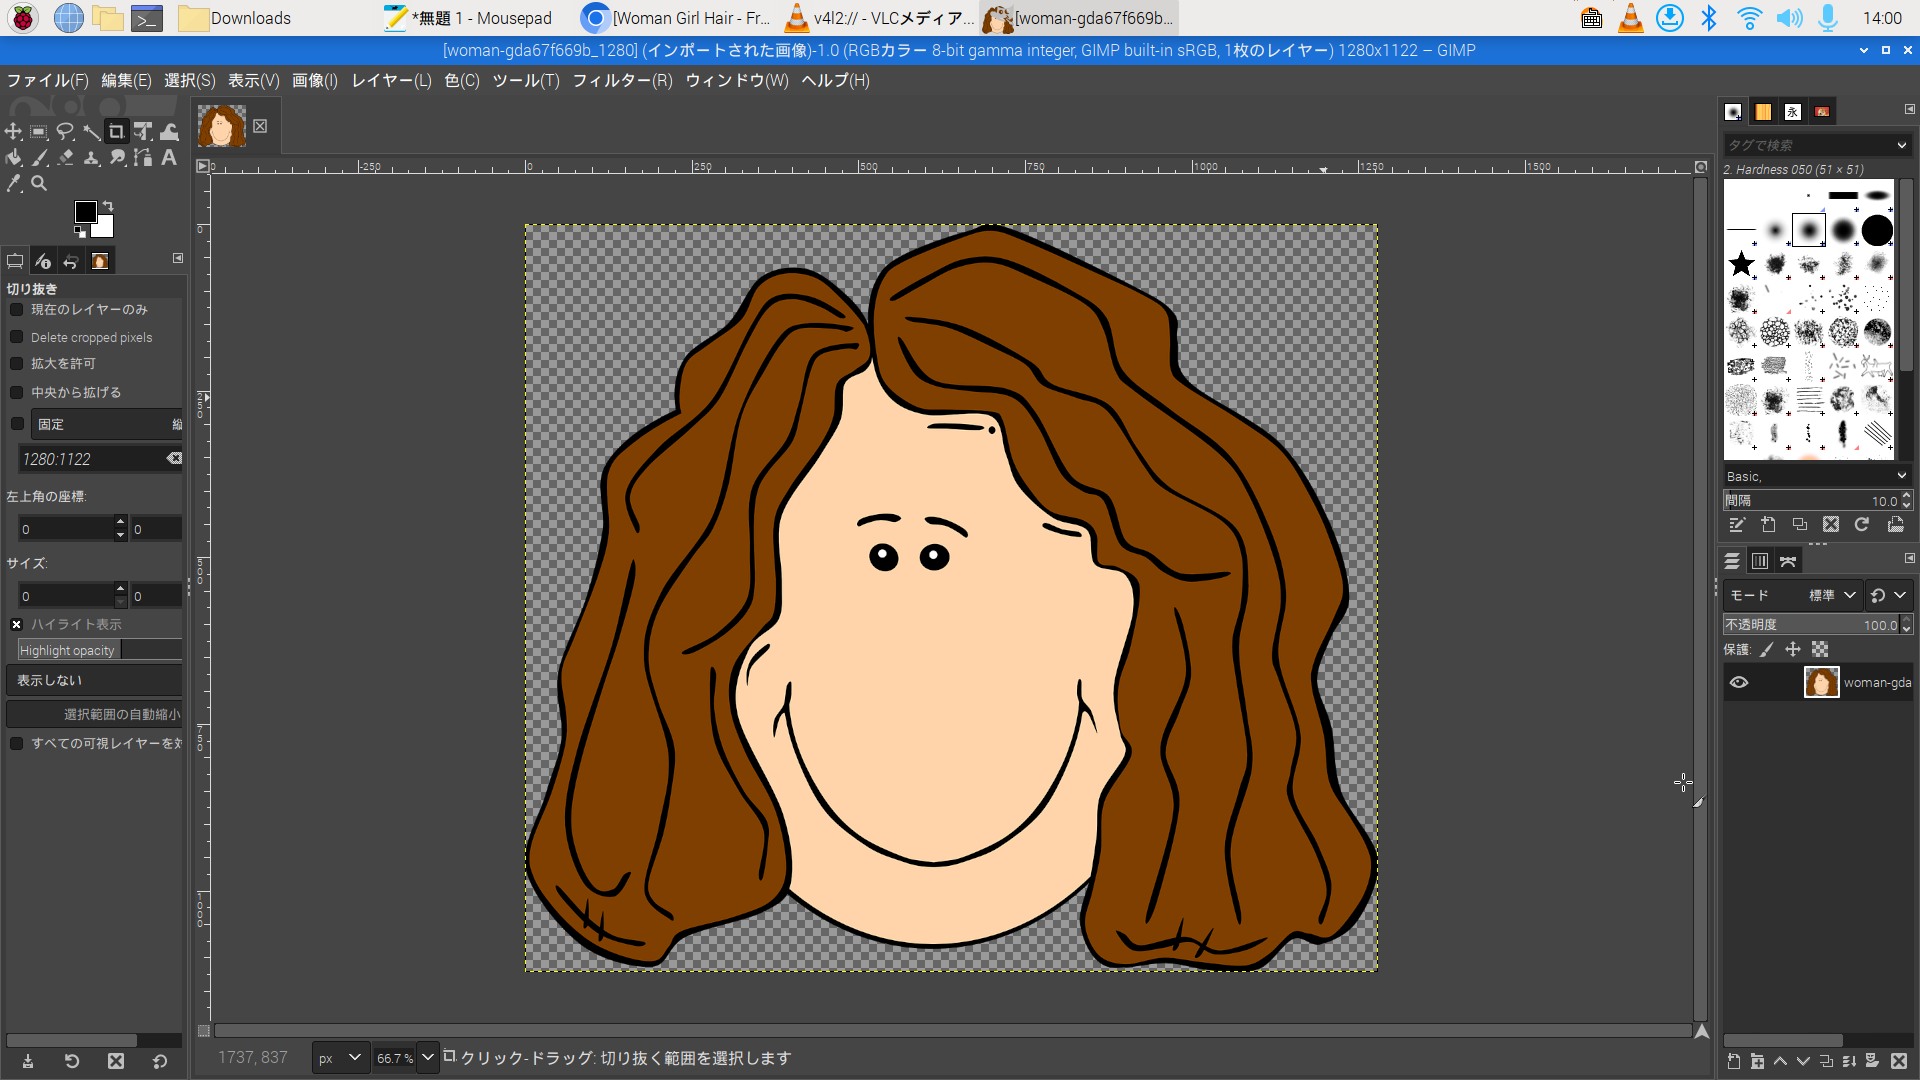
\includegraphics[width=\linewidth]{../../asset/image/textbook-img125.png}\\
    \textcircled{\scriptsize{2}} %
    \ruby{画像}{がぞう}\ruby{編集}{へんしゅう}モードになります
  \end{minipage}
  
  \begin{minipage}{0.4\textwidth}
    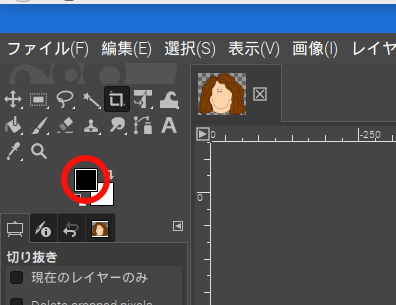
\includegraphics[width=\linewidth]{../../asset/image/textbook-img129.png}\\
    \textcircled{\scriptsize{3}} %
    画面左上の赤丸部分をクリック
  \end{minipage}
  \hspace{2cm}
  \begin{minipage}{0.4\textwidth}
    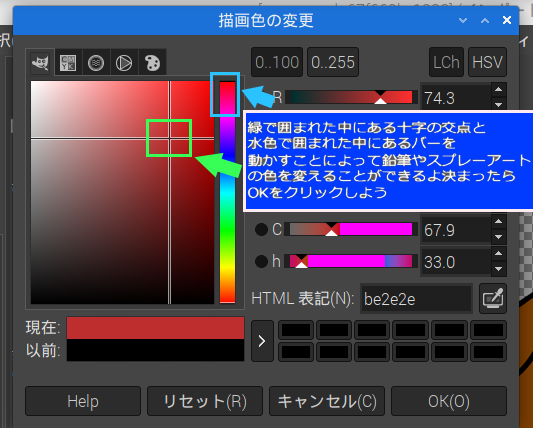
\includegraphics[width=\linewidth]{../../asset/image/textbook-img126.png}\\
    \textcircled{\scriptsize{4}} %
    好きな色を選んでOKを\ruby{押}{お}して色を選びましょう
  \end{minipage}

  \begin{minipage}{0.4\textwidth}
    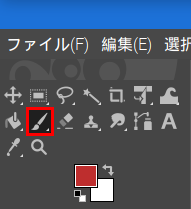
\includegraphics[width=\linewidth]{../../asset/image/textbook-img127.png}
    \textcircled{\scriptsize{5}} %
    赤わくのブラシアイコンをクリックすると、色付きの筆が使えるようになります
  \end{minipage}
  \hspace{2cm}
  \begin{minipage}{0.4\textwidth}
    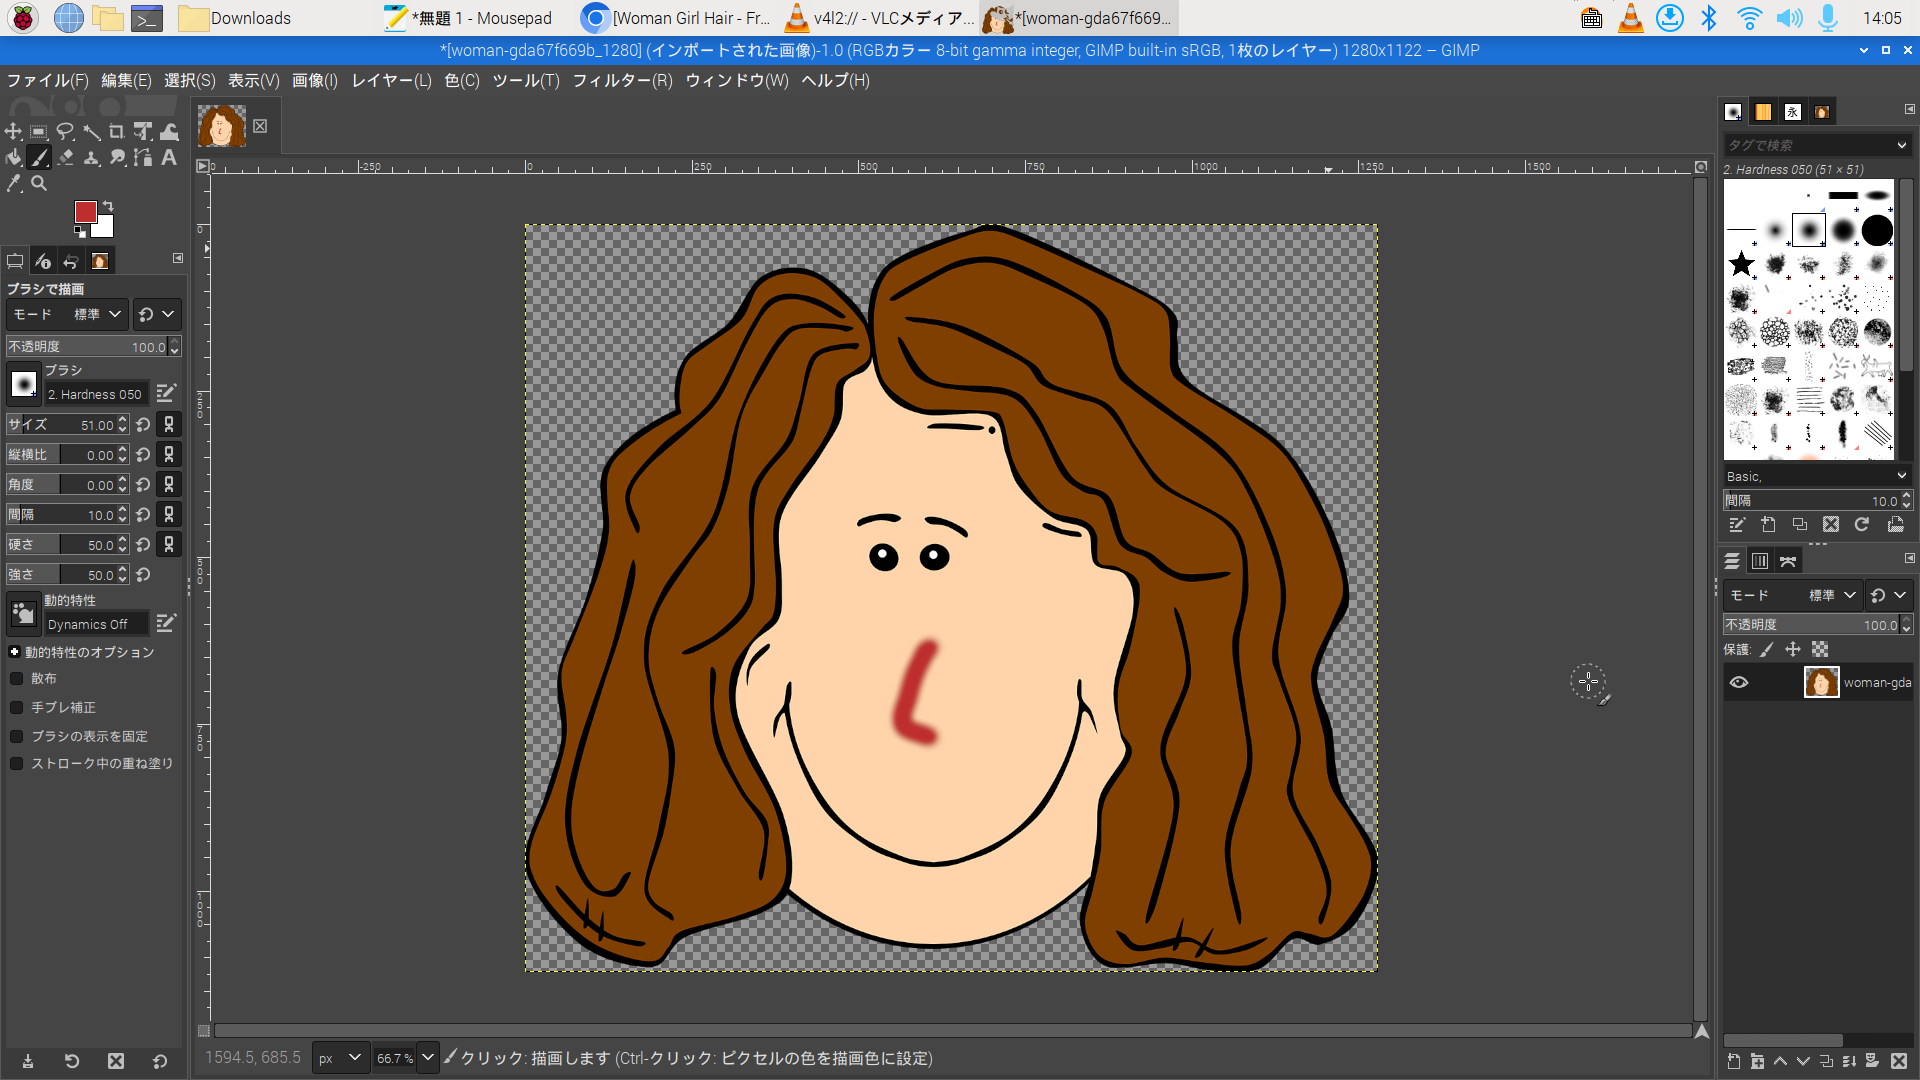
\includegraphics[width=\linewidth]{../../asset/image/textbook-img131.png}\\
    \textcircled{\scriptsize{6}} %
    左クリックをおしながら\ruby{画像}{がぞう}の上を\ruby{移動}{いどう}させると筆でお絵かきができますので、いたずら書きをしてみましょう
  \end{minipage}
\clearpage


    \begin{minipage}{0.47\textwidth}
      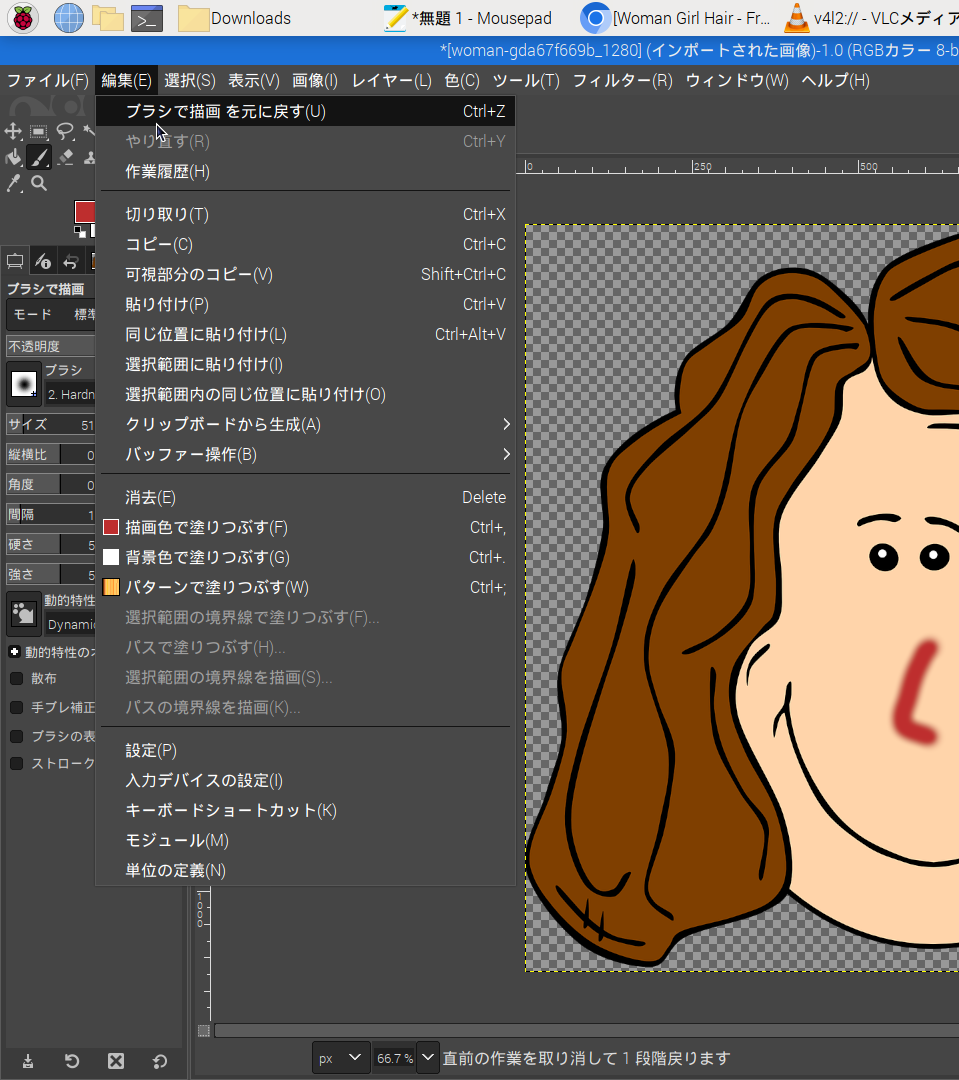
\includegraphics[width=0.95\linewidth]{../../asset/image/textbook-img132.png}\\
      \textcircled{\scriptsize{7}} %
      \ruby{間違}{まちが}えてしまって、もとに\ruby{戻}{もど}したいときは、メニューの\ruby{編集}{へんしゅう}からもとに\ruby{戻}{もど}すをクリックします
    \end{minipage}
    \hfill
    \begin{minipage}{0.47\textwidth}
      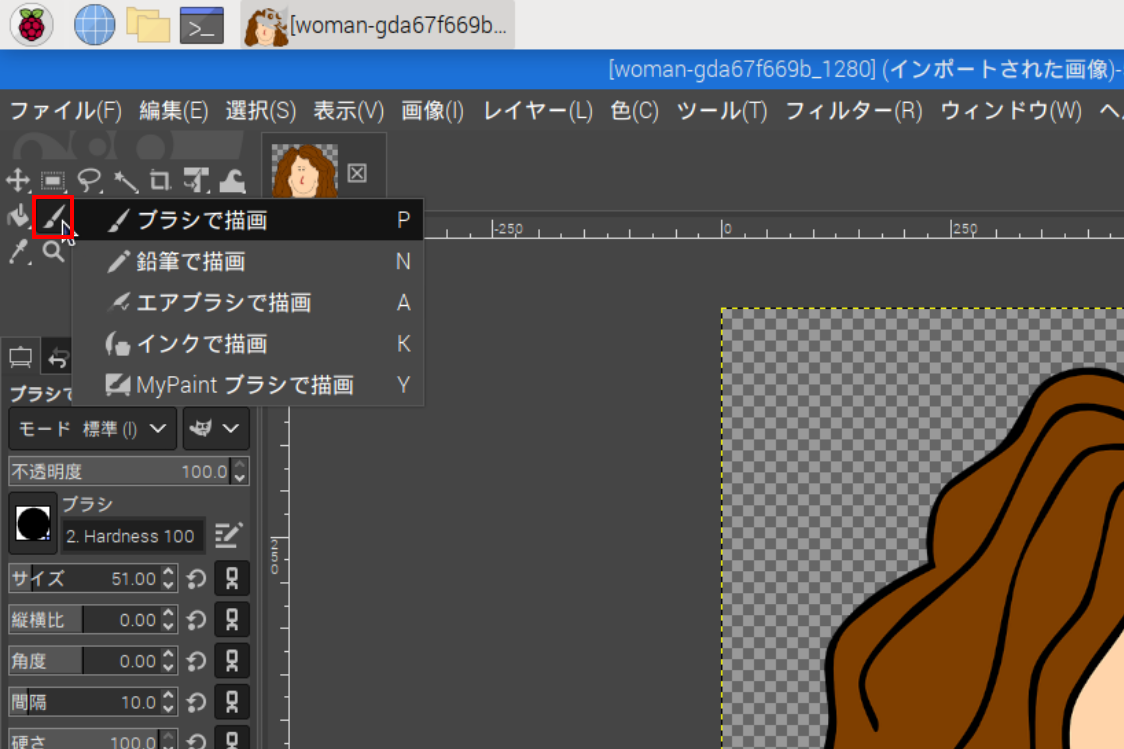
\includegraphics[width=0.95\linewidth]{../../asset/image/textbook-img133.png}\\
      \textcircled{\scriptsize{8}} %
      赤い\ruby{枠}{わく}で囲まれたブラシのアイコンを右クリックすると、別のブラシを選ぶことができます
      \ruby{鉛筆}{えんぴつ}やインクを試してみましょう。
    \end{minipage}
    \vspace{0.5cm}



\begin{minipage}{0.47\textwidth}
  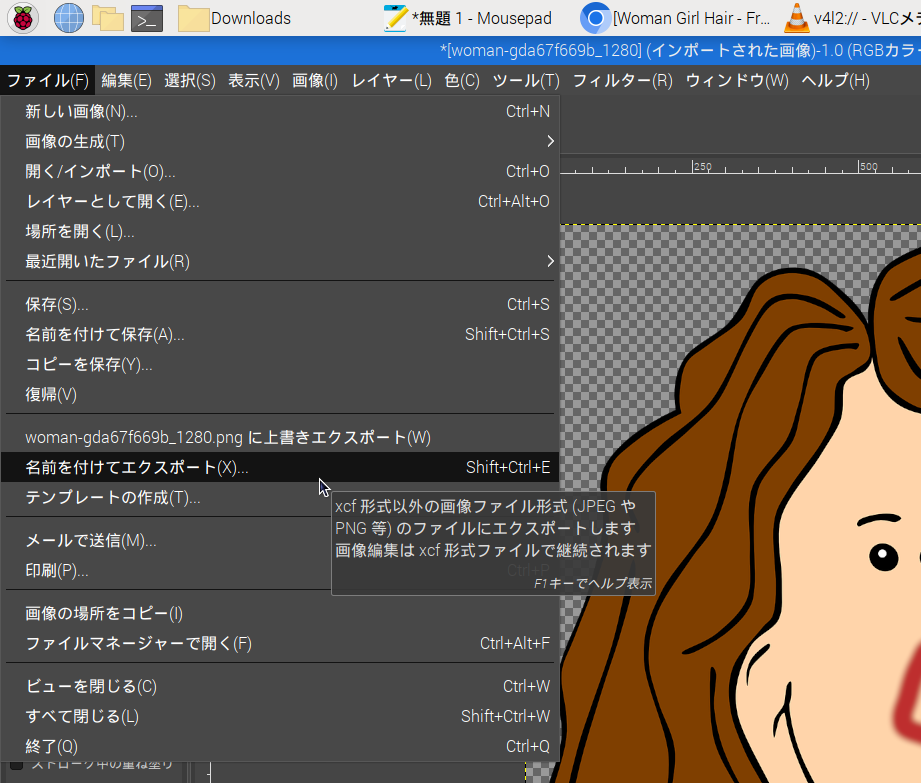
\includegraphics[width=0.95\linewidth]{../../asset/image/textbook-img138.png}\\
  \textcircled{\scriptsize{9}} %
  \ruby{編集}{へんしゅう}がおわったら、ファイルから名前を付けてエクスポートをクリックします
\end{minipage}
\hfill
\begin{minipage}{0.47\textwidth}
  % 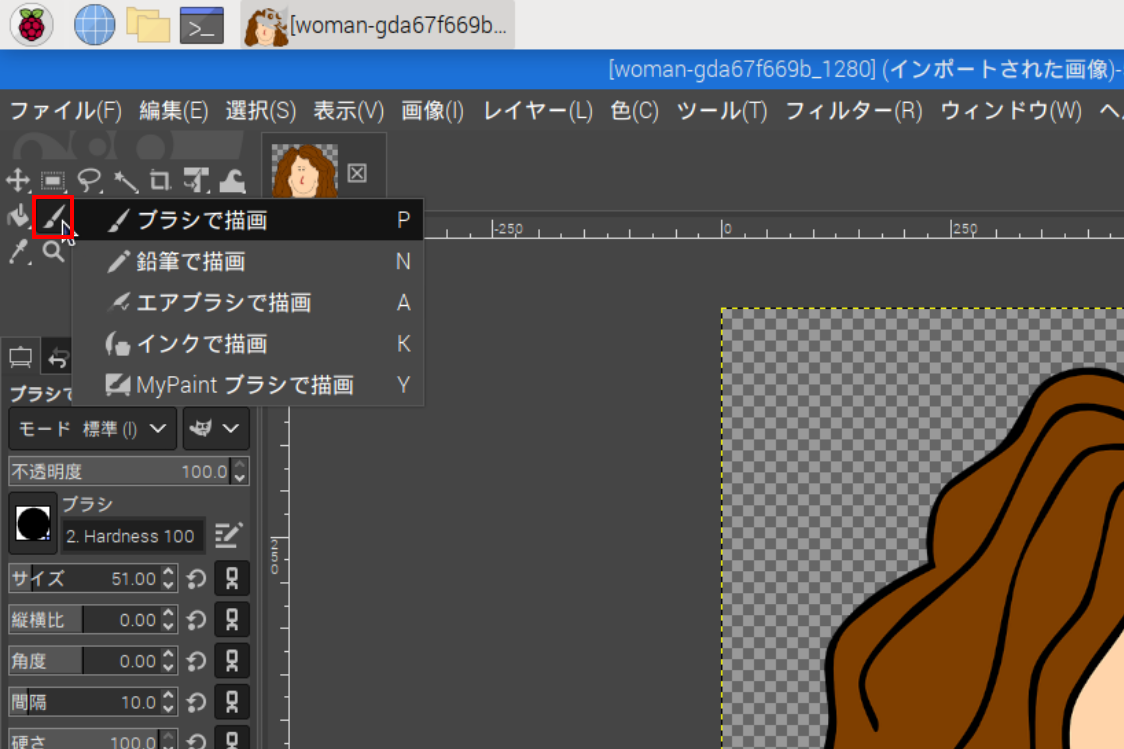
\includegraphics[width=8.881cm,height=4.997cm]{../../asset/image/textbook-img133.png}\\
  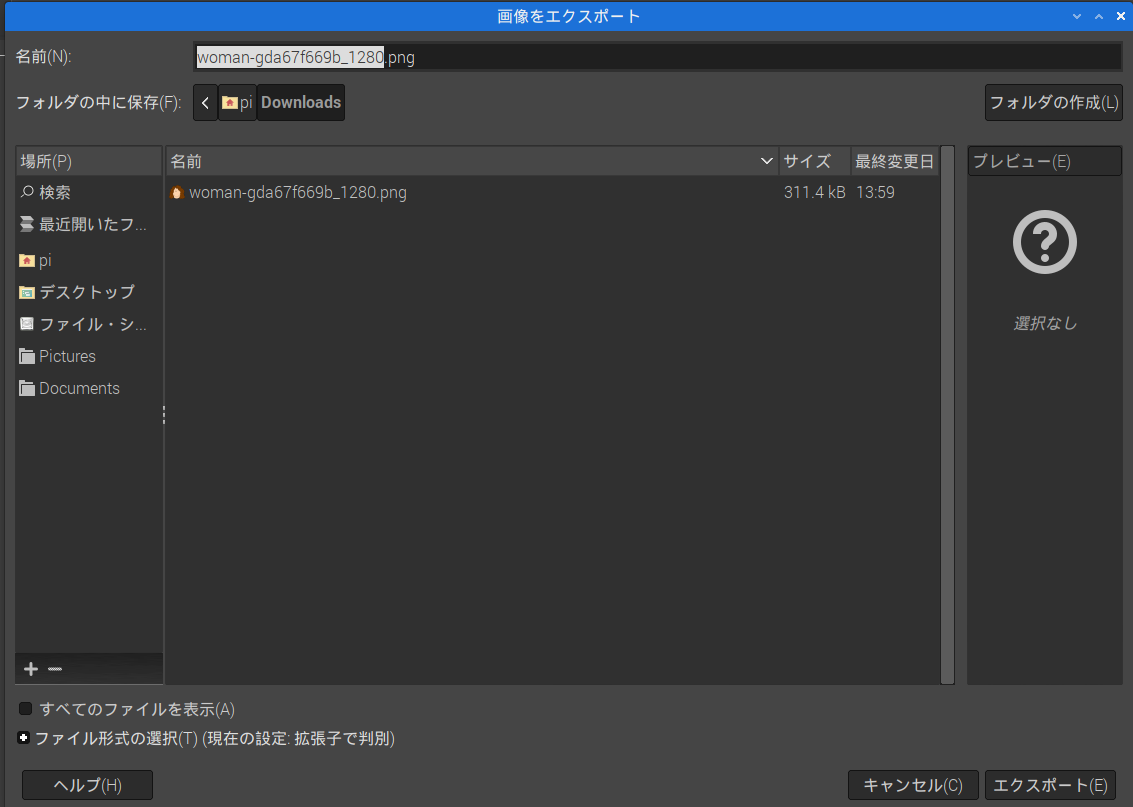
\includegraphics[width=0.95\linewidth]{../../asset/image/textbook-img137.png}\\
  \textcircled{\scriptsize{10}} %
  下のエクスポートをクリックします
\end{minipage}
\vspace{0.5cm}

\begin{minipage}{0.47\textwidth}
  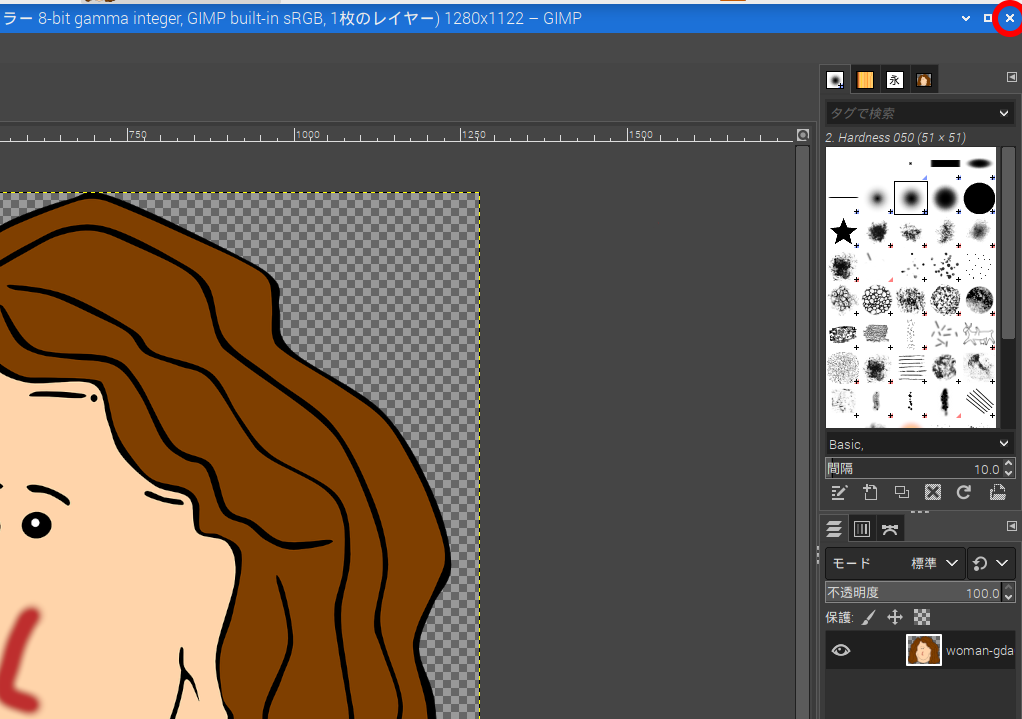
\includegraphics[width=0.95\linewidth]{../../asset/image/textbook-img1030.png}\\

  \textcircled{\scriptsize{11}} %
  GIMPを終了するには、右上の赤い丸で囲まれた×ボタンを\ruby{押}{お}します
\end{minipage}
\hfill
\begin{minipage}{0.47\textwidth}
  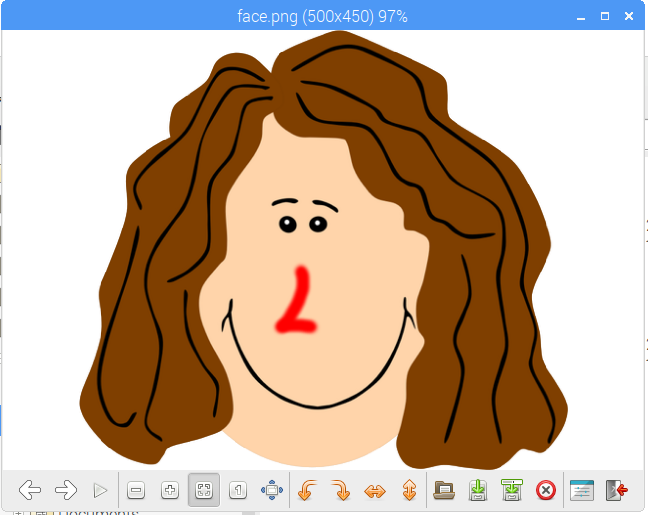
\includegraphics[width=0.9\linewidth]{../../asset/image/textbook-img139.png}\\
  \textcircled{\scriptsize{12}} %
\ruby{画像}{がぞう}ファイルを開いて\ruby{確認}{かくにん}してみましょう
\end{minipage}
\vspace{0.5cm}

\begin{tcolorbox}[title=\useOmetoi,breakable]
  \begin{enumerate}
    \addex{GIMPを使って、自分の顔写真にらくがきしてみましょう。}
    \addex{GIMPを使って、顔写真の下に、ブラシで名前を書いてみましょう。}
  \end{enumerate}
\end{tcolorbox}
\clearpage

\end{document}
